I'm trying a little bit of an experiment with a few projects of mine.

Advertising.

I am unashamed to admit that I run AdBlock almost all of the time that
I'm online. I think that advertising is a shoddy and cheap, albeit
necessary way for many online services to derive income, in general. I
also think that, in general, ads are effective on a level that is
perhaps not in line with the goals of an organization determined to be
as introspective as possible, in a lot of ways. That is, they don't
necessarily fit with the goal of the projects I have in mind. Flashy art
and animations are great for artists because they show off art and
animation skills. They're wonderful for organizations such as Rabbit
Valley and Sofawolf, that offer products for sale because they showcase
the products. Even so, I'm left with a few questions about the way
advertising works within the furry fandom, and how information is
transmitted within a potential audience.

How does one advertise a blog that offers nothing for sale and provides
a non-essential service?

How does one advertise for a survey, and in what ways does that impact
the results gained from that survey?

Does animation play a role? If so, how much?

What difference does wording make, particularly when it comes to key
words such as `sex'? For that matter, how does an advertisement that
mentions sex differ from an advertisement that does not?

These are hardly deep questions. Ask any advertising agency or the like
and you're likely to come up with some quips about what does and does
not work, as well as what works best for what type of product.

If you look at us, however, as well as our sister project, LSF, we are,
at best, irregularly-publishing magazines filled, almost entirely, with
opinion articles. The articles often have basis in statistics pulled
from here or there, but for the most part, the pieces are written more
as introspective or observational explorations of the act of
participating in a subculture. For us, these questions bear additional
meaning, as this advertising experiment is taking place almost entirely
within the subculture itself.

Here's what we've done:

\begin{enumerate}
\def\labelenumi{\arabic{enumi}.}
\tightlist
\item
  I've set up four advertisements on two different sites, FurAffinity
  and SoFurry. These ads are for four different projects:
  {[}adjective{]}{[}species{]}, \href{http://lovesexfur.com}{Love - Sex
  - Fur}, \href{http://furrypoll.com}{The Furry Survey}, and an
  unrelated project, \href{http://bookmarfs.com}{Bookmarfs!}.
\item
  All four advertisements have slight differences:

  \begin{itemize}
  \tightlist
  \item
    All ads except for Bookmarfs! are animated.
  \item
    The ad for LSF contains the word `sex'.
  \item
    The ad for {[}a{]}{[}s{]} and for the Furry Survey contain text
    other than the subtitle of the site.\\
  \end{itemize}
\item
  The ads should rotate fairly evenly among other ads on both sites
  (though Dragoneer and Tourmal are invited to comment on the
  advertising systems in place on their respective sites).
\item
  All four ads have campaign data indicating their source. These only
  show up once per click, of course, so we'll only see these as unique
  visitors. That is, there's no way to bolster the numbers by simply
  clicking on the ads a bunch of times!
\end{enumerate}

Just to start things out, I've taken snapshots from before the ads went
up of how traffic looks.

\subsection{{[}adjective{]}{[}species{]}}\label{adjectivespecies}

\begin{figure}[htbp]
\centering
\includegraphics{/assets/furry/ads/adjspecies.gif}
\caption{{[}adjective{]}{[}species{]} ad}
\end{figure}

\begin{figure}[htbp]
\centering
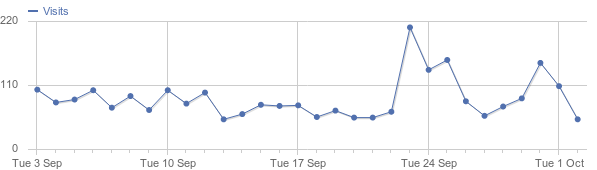
\includegraphics{/assets/furry/ads/as-preads.png}
\caption{{[}adjective{]}{[}species{]} pre-ads}
\end{figure}

You can see, here, just how the traffic generally looks for this site in
particular. You can see, for example, when articles go live, and even
when an article that winds up becoming particularly popular or
contentious goes live as compared to one that doesn't: JM published an
article on introversion on Monday the 23rd that became the subject of
heated discussion, and I published an article two days later that was
largely neutral (this is the way of things, we've decided: I write
introspective pieces, JM writes more provocative pieces). This is a
pretty standard few weeks for us, and we've had few deviations from
that. One can see the effects from conventions at which we have panels
or advertising, as we did for Anthrocon one year.

\subsection{Love - Sex - Fur}\label{love---sex---fur}

\begin{figure}[htbp]
\centering
\includegraphics{/assets/furry/ads/lovesexfur.gif}
\caption{Love - Sex - Fur ad}
\end{figure}

\begin{figure}[htbp]
\centering
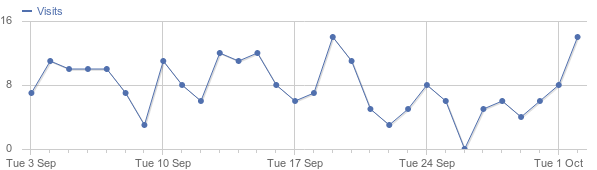
\includegraphics{/assets/furry/ads/lsf-preads.png}
\caption{Love - Sex - Fur pre-ads}
\end{figure}

LSF has been quiet of late, due to my personal schedule, and so you can
see a similar graph, lower in traffic, to the time between articles on
this site. Visitors come in from various places, usually search engines
and old Twitter links (the t.co link-shortener shows up as the referrer
in these cases).

\subsection{The Furry Poll}\label{the-furry-poll}

\begin{figure}[htbp]
\centering
\includegraphics{/assets/furry/ads/furrypoll.gif}
\caption{The Furry Poll ad}
\end{figure}

\begin{figure}[htbp]
\centering
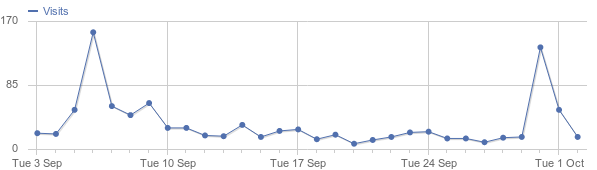
\includegraphics{/assets/furry/ads/furrypoll-preads.png}
\caption{The Furry Poll pre-ads}
\end{figure}

The Furry Poll, not having any changes over time within the year, shows
bumps primarily from links in from outside, such as on this site, or
other forums where others post the link. Reddit, FurAffinity forums,
FurBase.de, and so on are all sources of the second bump, for example.

\subsection{Bookmarfs!}\label{bookmarfs}

\begin{figure}[htbp]
\centering

\includegraphics{/assets/furry/ads/bookmarfs.png}
\caption{Bookmarfs! ad}
\end{figure}

\begin{figure}[htbp]
\centering
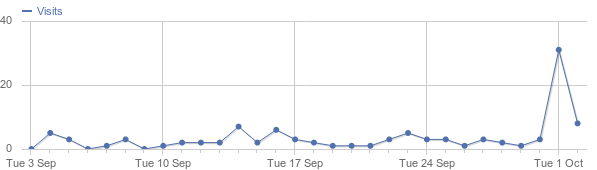
\includegraphics{/assets/furry/ads/bookmarfs-preads.png}
\caption{Bookmarfs! pre-ads}
\end{figure}

Bookmarfs!, on the other hand, gains traffic at regular intervals from
posts at the beginning of the month (when that month's book is
announced), and at the end of the month (when that month's discussion
occurs). Full disclosure: although Bookmarfs! is not related to
{[}a{]}{[}s{]} at all, I do help out with them in a technical capacity.

You can also see the advertisements that we placed, above. These are the
different paths that we'll be investigating as inroads that advertising
provides. What it is that we hope to see is how information spreads
within the fandom in terms of something sort of neutral and random such
as these advertisements, organic social sharing, such as retweets or
links provided to friends, and from followers who catch us on FA
journals, Tweets, or G+ posts.

Working within a subculture such as ours, I will posit that, while
advertising drives some traffic to sites such as these, the majority of
our readership found the site through sharing, due to the nature of our
content. However, given that these ads will all be live for about a
month, I'll pull statistics again in a few weeks and see just how things
have changed - or not!

We're interested to hear how you found this site (and if you found the
others, how), as well as how \emph{you} think that this little
experiment will play out. Will members of the furry community pay
attention to the ads? Will they largely ignore them? How do you feel
about advertising in general, and on furry sites? Do you treat them
differently? Let us know in the comments!

(Note: {[}a{]}{[}s{]} and related projects are, of course, run totally
out of pocket, and we have no ad revenue of our own; we stand to gain
nothing but information from this little experiment, all of which we aim
to share with you!)
